\chapter{Análisis de riesgos}

Para el análisis de los riesgos del proyecto, se ha decidido utilizar la estrategia de Mitigación y Gestión de Riesgos, conocido por sus siglas en inglés como RMMM (Risk Mitigation, Monitoring and Management). Para llevar a cabo cada una de las tareas anteriormente mencionadas, se ideará un plan de prevención, un plan de monitorización y un plan de contingencia respectivamente.

\begin{figure}[H]
   \centering
   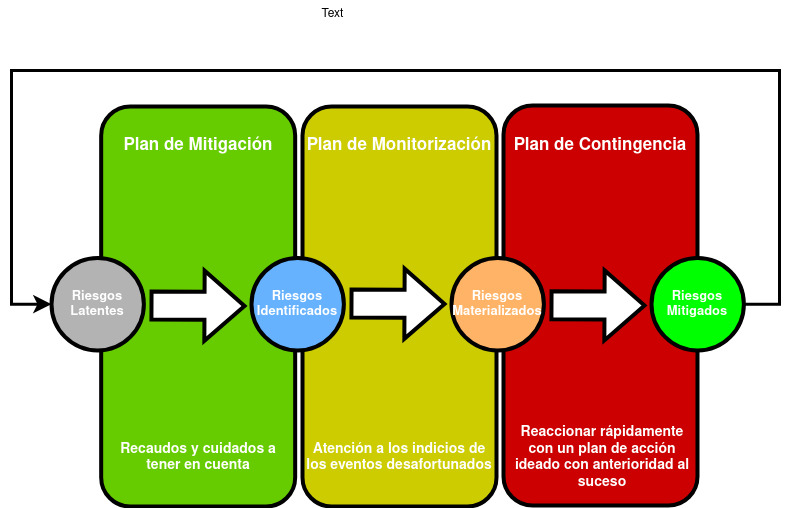
\includegraphics[trim={0 0 0 2cm}, clip, width=0.8\linewidth]{images/rmmm.jpg}
   \caption{Estrategia de Mitigación, Monitorización y Gestión de riesgos}
   \label{fig:rmmm}
\end{figure}

Se consideran riesgos aquellas situaciones que, en caso de suceder, afectan negativamente determinados aspectos del proyecto. Por esta razón es importante identificarlos con anticipación para mitigarlos.

El plan de prevención intenta ser un escudo para mantener la cantidad de riesgos latentes al mínimo y que no logren materializarse, por lo que su objetivo es entorpecer lo máximo posible el flujo a través del circuito RMMM.

El plan de monitorización busca detectar tempranamente las situaciones que pueden desencadenar la materialización de un riesgo en particular, para poder evitar en caso de ser posible, que se concrete el riesgo.

El plan de contingencia hace la gestión del riesgo, es decir, que una vez que se concreta un evento desafortunado asociado a un riesgo, se procede inmediatamente a solucionarlo y luego poder continuar con el proyecto. Las soluciones en esta etapa no deben ser tomadas apresuradamente porque pueden incrementar el nivel de riesgos de todo el proyecto y hacerlo inestable. \cite{rmmm}

La ponderación de riesgos será calculada en base a la siguiente ecuación:

\begin{equation}
    Estimaci\acute{o}n\ de\ la\ probabilidad \times Estimaci\acute{o}n\ del\ impacto = Exposici\acute{o}n\ al\ riesgo
\end{equation}

\section{Listado de riesgos}

\begin{table}[H]
\centering
\begin{tabular} {|m{2.5cm}|m{11.5cm}|}
    \hline \rowcolor{test_header_color}
    RI-01 & Incompatibilidad o avería de componentes \\
    \hline
        Condición & Elección incorrecta del sistema embebido a usar. \\
    \hline
        Consecuencias & Interrupciones en el funcionamiento del robot, comportamiento errático, pérdida de enlaces de comunicación, reinicios inesperados, entre otros. \\
    \hline
        Efecto & No se logrará cumplir con las expectativas mínimas de robustez y estabilidad que se espera de un robot autónomo. \\
    \hline
\end{tabular}
\label{}
\caption{Incompatibilidad o avería de componentes}
\end{table}

\begin{table}[H]
\centering
\begin{tabular} {|m{2.5cm}|m{11.5cm}|}
    \hline \rowcolor{test_header_color}
    RI-02 & Intercomunicación de componentes ineficiente o ineficaz \\
    \hline
        Condición & Comunicación entre componentes lenta, con interferencias y/o con ruido. \\
    \hline
        Consecuencias & Sistema robótico con tiempo de respuestas grandes que imposibilitan un eficaz funcionamiento de un sistema de control. \\
    \hline
        Efecto & El robot no podrá reaccionar a tiempo para evitar obstáculos que detecte en su camino y podrá desviarse del camino. Las respuestas del robot a los comandos de movimientos están muy desfasadas en el tiempo, lo que dificultará su manejo tanto manual como autónomo. A tiempo de respuesta mayores, menor será la velocidad máxima permitida de desplazamientos del robot. \\
    \hline
    \end{tabular}
\caption{Intercomunicación de componentes ineficiente o ineficaz}
\end{table}

\begin{table}[H]
\centering
\begin{tabular} {|m{2.5cm}|m{11.5cm}|}
    \hline \rowcolor{test_header_color}
    RI-03 & Prestaciones insuficientes de componentes \\
    \hline
        Condición & Sobrestimar las especificaciones técnicas de componentes. También puede ocurrir subestimar las necesidades tecnológicas de la solución. Falta documentación fiable de componentes. \\
    \hline
        Consecuencias & Componentes que no son capaces de cumplir correctamente con su propósito y por lo tanto pasan a ser inservibles para los fines del proyecto. \\
    \hline
        Efecto & Incremento del costo económico del proyecto por el descarte y reemplazo de los componentes por otros de mayor prestaciones. \\
    \hline
\end{tabular}
\caption{Prestaciones insuficientes de componentes}
\end{table}

\begin{table}[H]
\centering
\begin{tabular} {|m{2.5cm}|m{11.5cm}|}
    \hline \rowcolor{test_header_color}
    RI-04 & Modificación de los requerimientos del proyecto \\
    \hline
        Condición & Definición de nuevos requisitos o modificaciones de los existentes durante el desarrollo del proyecto. \\
    \hline
        Consecuencias & Replanificación de las tareas a realizar. Desarrollos en etapas avanzadas en los que sí invirtió tiempo y esfuerzo pueden interrumpirse y quedar inservibles para los fines del proyecto. \\
    \hline
        Efecto & Retrasos en la finalización del producto final del proyecto. \\
    \hline
\end{tabular}
\caption{Modificación de los requerimientos del proyecto}
\end{table}

\begin{table}[H]
\centering
\begin{tabular} {|m{2.5cm}|m{11.5cm}|}
    \hline \rowcolor{test_header_color}
    RI-05 & Dificultad en conseguir determinados componentes \\
    \hline
        Condición & Componentes electrónicos que deben ser importados y provenientes de empresas que no trabajan con envíos al exterior. Altos costos de importación y/o envío. Grandes tiempo de demora en los envíos desde el exterior. \\
    \hline
        Consecuencias & Análisis de componentes alternativos que puedan ser utilizados para el mismo fin que el componente que no puede conseguirse. En última instancia podrían adaptarse los requerimientos del proyecto. \\
    \hline
        Efecto & Retrasos en la finalización del producto final del proyecto y/o degradación de las capacidades del robot. \\
    \hline
\end{tabular}
\caption{Dificultad en conseguir determinados componentes}
\end{table}

\begin{table}[H]
\centering
\begin{tabular} {|m{2.5cm}|m{11.5cm}|}
    \hline \rowcolor{test_header_color}
    RI-06 & Excesivo tiempo para cumplir los objetivos del proyecto \\
    \hline
        Condición & Cualquier dificultad técnica que retrase significativamente el progreso del proyecto. Escasez de tiempo disponible de los integrantes del equipo de desarrollo \\
    \hline
        Consecuencias & Robot con capacidades reducidas, menores a las esperadas. \\
    \hline
        Efecto & Directores del proyecto podrán readaptar los objetivos a alcanzar dando una extensión de tiempo más allá de lo planificado desde un comienzo. \\
    \hline
\end{tabular}
\caption{Excesivo tiempo para cumplir los objetivos del proyecto}
\end{table}

\begin{table}[H]
\centering
\begin{tabular} {|m{2.5cm}|m{11.5cm}|}
    \hline \rowcolor{test_header_color}
    RI-07 & Reducción de la fuerza de trabajo \\
    \hline
        Condición & Miembros del equipo que abandonen el proyecto. \\
    \hline
        Consecuencias & Las tareas a realizar llevaran más tiempo concretarlas. \\
    \hline
        Efecto & Retraso en la entrega final del proyecto. \\
    \hline
\end{tabular}
\caption{Reducción de la fuerza de trabajo}
\end{table}

\section{Estimación de la probabilidad}

En la siguiente tabla se expone los criterios en base a los cuales se cuantificará la probabilidad de ocurrencia de los riesgos anteriormente mencionados.
\begin{table}[H]
\centering
\begin{tabular}{
    | >{\centering\arraybackslash}m{2cm}
    | >{\centering\arraybackslash}m{3cm}
    | >{\centering\arraybackslash}m{4cm}
    | >{\centering\arraybackslash}m{1.5cm}
    | >{\centering\arraybackslash}m{1.5cm} |
    }
    \hline \rowcolor{test_header_color}
        Rango de probabilidad & Promedio para el cálculo & Expresión en lenguaje natural & Valor numérico & Código de color \\
    \hline
        1\% a 20\% & 10\% & Muy baja probabilidad & 1 & \cellcolor{blue!65}\\
    \hline
        21\% a 40\% & 30\% & Baja probabilidad & 2 & \cellcolor{green!65}\\
    \hline
        41\% a 60\% & 50\% & Mediana probabilidad & 3 & \cellcolor{yellow!65}\\
    \hline
        61\% a 80\% & 70\% & Alta probabilidad & 4 & \cellcolor{orange!65}\\
    \hline
        81\% a 99\% & 90\% & Muy alta probabilidad & 5 & \cellcolor{red!65}\\
    \hline
\end{tabular}
\caption{Cuantificación de la probabilidad}
\end{table}

\newpage
A continuación se expresan los riesgos identificados para el proyecto con las probabilidades estimadas subjetivamente.
\begin{table}[H]
\centering
\begin{tabular} {
    | >{\centering\arraybackslash}m{1cm}
    | >{\centering\arraybackslash}m{9cm}
    | >{\centering\arraybackslash}m{2.9cm} |
    }
    \hline \rowcolor{test_header_color}
        ID & Riesgo & Probabilidad \\
    \hline
        RI-01 & Incompatibilidad o avería de componentes & Mediana \cellcolor{green!65}\\
    \hline
        RI-02 & Intercomunicación de componentes ineficiente o ineficaz & Alta \cellcolor{yellow!65}\\
    \hline
        RI-03 & Prestaciones insuficientes de componentes & Mediana \cellcolor{orange!65}\\
    \hline
        RI-04 & Modificación de los requerimientos del proyecto & Baja \cellcolor{green!65}\\
    \hline
        RI-05 & Dificultad en conseguir determinados componentes & Muy alta \cellcolor{red!65}\\
    \hline
        RI-06 & Excesivo tiempo para cumplir los objetivos del proyecto & Alta \cellcolor{orange!65}\\
    \hline
        RI-07 & Reducción de la fuerza de trabajo & Muy baja \cellcolor{blue!65}\\
    \hline
\end{tabular}
\caption{Probabilidad de ocurrencia de riesgos}
\end{table}

\section{Estimación de impacto}

En la siguiente tabla se expresa los criterios en base a los cuales se cuantificará el impacto de los riesgos.
\begin{table}[H]
\centering
\begin{tabular} {
    | >{\centering\arraybackslash}m{3cm}
    | >{\centering\arraybackslash}m{5cm}
    | >{\centering\arraybackslash}m{1.5cm}
    | >{\centering\arraybackslash}m{1.5cm} |
    }
    \hline \rowcolor{test_header_color}
        Criterio & Retraso en la planificación & Valor numérico & Código de color \\
    \hline
        Insignificante & 1 semana & 1 & \cellcolor{blue!65} \\
    \hline
        Moderado & 2 a 3 semanas & 2 & \cellcolor{green!65} \\
    \hline
        Medio & 4 a 5 semanas & 3 & \cellcolor{yellow!65} \\
    \hline
        Crítico & 6 a 8 semanas & 4 & \cellcolor{orange!65} \\
    \hline
        Catastrófico & Más de 8 semanas & 5 & \cellcolor{red!65} \\
    \hline
\end{tabular}
\caption{Cuantificación del impacto de los riesgos}
\end{table}

En la próxima tabla se expone el impacto estimado en cuanto al máximo tiempo que puede provocar la efectivización de un riesgo en el peor de los casos.
\begin{table}[H]
\centering
\begin{tabular}{|c|c|c|}
    \hline \rowcolor{test_header_color}
        ID & Riesgo & Impacto \\
    \hline
        RI-01 & Incompatibilidad o avería de componentes & Moderado \cellcolor{green!65} \\
    \hline
        RI-02 & Intercomunicación de componentes ineficiente o ineficaz & Moderado \cellcolor{yellow!65} \\
    \hline
        RI-03 & Prestaciones insuficientes de componentes & Medio \cellcolor{yellow!65} \\
    \hline
        RI-04 & Modificación de los requerimientos del proyecto & Medio \cellcolor{orange!65} \\
    \hline
        RI-05 & Dificultad en conseguir determinados componentes & Crítico \cellcolor{orange!65} \\
    \hline
        RI-06 & Excesivo tiempo para cumplir los objetivos del proyecto & Catastrófico \cellcolor{red!65} \\
    \hline
        RI-07 & Reducción de la fuerza de trabajo & Crítico \cellcolor{orange!65} \\
    \hline
\end{tabular}
\caption{Impacto en base a los diferentes riesgos}
\end{table}

\newpage
\section{Exposición al riesgo}

En esta tabla se visibiliza la exposición del riesgo de cada uno de los requerimientos.
\begin{table}[H]
\centering
\begin{tabular} {
    | >{\centering\arraybackslash}m{1cm}
    | >{\centering\arraybackslash}m{7cm}
    | >{\centering\arraybackslash}m{2cm}
    | >{\centering\arraybackslash}m{1.4cm}
    | >{\centering\arraybackslash}m{1.6cm} |
    }
    \hline \rowcolor{test_header_color}
        ID & Riesgo & Probabilidad & Impacto & Exposición \\
    \hline
        RI-01 & Incompatibilidad o avería de componentes & 50\%\cellcolor{yellow!65} & 2 \cellcolor{green!65} & 1 \\
    \hline
        RI-02 & Intercomunicación de componentes ineficiente o ineficaz & 70\%\cellcolor{orange!65} & 2\cellcolor{orange!65} & 2,1\\
    \hline
        RI-03 & Prestaciones insuficientes de componentes & 50\%\cellcolor{yellow!65} & 3 \cellcolor{yellow!65}& 1,5 \\
    \hline
        RI-04 & Modificación de los requerimientos del proyecto & 30\%\cellcolor{green!65} & 4 \cellcolor{orange!65} & 1,2 \\
    \hline
        RI-05 & Dificultad en conseguir determinados componentes & 90\%\cellcolor{red!65} & 4 \cellcolor{orange!65} & 3,6 \\
    \hline
        RI-06 & Excesivo tiempo para cumplir los objetivos del proyecto & 70\%\cellcolor{orange!65} & 5\cellcolor{red!65} & 3,5 \\
    \hline
        RI-07 & Reducción de la fuerza de trabajo & 10\%\cellcolor{blue!65} & 4\cellcolor{orange!65} & 0,4 \\
    \hline
\end{tabular}
\caption{Exposición al riesgo}
\end{table}

\section{Conclusión}
El análisis de riesgos presentado permite identificar y priorizar los principales desafíos que podrían afectar el desarrollo del proyecto. Mediante la implementación de los planes de prevención, monitoreo y contingencia, se busca mitigar el impacto de estos riesgos, garantizando que el proyecto avance de manera estable y eficiente. La ponderación de riesgos mediante la ecuación de exposición al riesgo facilitará la toma de decisiones informadas y la asignación adecuada de recursos, contribuyendo al éxito del proyecto.